%!TEX root = main.tex
\chapter{Dataset}
På de følgende sider vil vi gennnemgå vores dataset. Vi vil vise de basale statistikker over dataet for hver af de perioder vi har arbejdet med og gennemgå afvigelser. Vi vil også gennemgå hvordan vi forholder os til disse afvigelser og hvordan vi lavede datacleaning. \\
Til sidst vil vi runde afsnittet af med en del-konlusion. 

Vores data stammer fra Sony's Lifelog\cite{sonyLifeLog} som, navnet antyder, er en mobil Lifelog app som logger ens aktiviteter i løbet af dagen. Heri logger den bla. aktivitet i apps og geolokation. Vores dataset stammer fra denne app, indsamlet fra Sony medarbejdere og, som det fremkommer senere, henover forskellige perioder i 2015. % over 3 måneder\footnote{September 2015 - November 2015} fordelt på 80 lande. 

Vi har valgt at dele datasættet op i to dele, for overblikkets skylde: En \textbf{geolokation del} og en \textbf{app og homophily del}.

\section{Geolokation del}
Denne del af datasættet beskriver geolokationerne for hvor en bruger har været. Det beskriver præcis hvor, hvornår og hvor længe brugeren har været det pågældende sted. Hver gang brugeren skifter lokation (defineret ud fra latitude og longitude), bliver der logget en lokations opdatering med følgende oplysninger:
\begin{enumerate}
\item \texttt{\textbf{timestamp\_seen}}\\Millisekunder siden brugerens systems epoch, da den pågældende lokations opdatering bliver logget. 
\item \texttt{\textbf{id}}\\Lokations id repræsenteret som en streng. 
\item \texttt{\textbf{useruuid}}\\Brugerens unikke id repræsenteret som en streng
\item \texttt{\textbf{start\_time}}\\Tid for hvornår brugeren går ind i en lokation. Repræsenteret som ISO8601 time stamp med timezone
\item \texttt{\textbf{end\_time}}\\Tid for hvornår brugeren går ud af en lokation. Repræsenteret som ISO8601 time stamp med timezone
\item \texttt{\textbf{name}}\\Navnet på byen hvor brugeren befinder sig, når lokations opdateringen bliver logget
\item \texttt{\textbf{area}}\\Navnet på området hvor brugeren befinder sig, når lokations opdateringen bliver logget. F.eks. Skåne i Sverige
\item \texttt{\textbf{country}}\\Navnet på landet hvor brugeren befinder sig, når lokations opdateringen bliver logget
\item \texttt{\textbf{region}}\\Navnet på regionen hvor brugeren befinder sig, når lokations opdateringen bliver logget. F.eks. EU
\item \texttt{\textbf{latitude}}\\Latitude for lokationen. Latitude har en præcition på ca 15 cifre, hvilket svarer til 0.1 nanometer \textcolor{red}{[KILDE!!!]}. Denne præcition er skal man dog ikke tage så højtidligt, da de fleste mobil GPS'er har en fejl margen på maks 30 meter \cite{NAV:8292634}.  
\item \texttt{\textbf{longitude}}\\Longitude for lokationen. Latitude har en præcition på ca 15 cifre, hvilket svarer til 0.1 nanometer. Vedr. præcition, gælder det samme som ved latitude
\item \texttt{\textbf{altitude}}\\Altitude repræsenteret i mm. Dette bliver beregnet af telefonens gyroskop samt GPS
\item \texttt{\textbf{accuracy}}\\Accuracy repræsenteret i mm. Accuracy er hvor nøjagtigt man kan regne med GPS'en er i den pågældene lokations opdatering. Værdien fortæller at brugeren med sikkerhed er i pågældende sted, indenfor denne distance som accuracy er. Jo lavere værdi, jo bedre. Dette styres af telefonens styresystem og GPS
\item \texttt{\textbf{devices}}\\Devices er repræsentet som et array med name, type og id. Type er hvilken type device (f.eks. Phone), name er navnet på det device og id er devices unikke id. 
\end{enumerate}

Nogle af overstående oplysninger er ikke relevante for vores problemstilling. Dette gør vi kan skære disse fra og vi ender dermed at have følgende oplysninger (fra nu af kaldt  attributter) at arbejde med: 

\begin{itemize}
\item \texttt{useruuid}
\item \texttt{start\_time}
\item \texttt{end\_time}
\item \texttt{name}
\item \texttt{area}
\item \texttt{country}
\item \texttt{region}
\item \texttt{latitude}
\item \texttt{longitude}
\item \texttt{altitude}
\item \texttt{accuracy}
\end{itemize}

Disse oplysinger har vi valgt, da de mere eller mindre er vigtige eller interssante i forhold til vores problemstilling. \texttt{useruuid} er vigtig for at kunne skelne brugerene fra hinanden, \texttt{start\_time} og \texttt{end\_time} er vigtige, da de fortæller hvornår/hvor længe brugeren har været i den pågældende lokation. \texttt{country} er til nemt at kunne filtrere brugerene, hvor \texttt{name}, \texttt{area} og \texttt{region}, ikke er særlige vigtige men kunne være interessant at kigge på. \texttt{latitude} og \texttt{longitude} er meget væsentlige, da de fortæller nok det mest vigtigste, nemlig hvilken lokation brugeren befinder sig. \texttt{accuracy} kan fortælle os i for høj grad vi kan bruge den pågældene lokations opdatering, mens \texttt{altitude} kunne være interessant at at kigge på mht. fin-filtrering. 

Vi har kigget på data fra en test periode og herefter alt data som Sony havde på daværende tidspunkt (production data). Vi vil beskrive hvordan henholdsvis test perioden og production data ser ud mht. distributioner mm. 

\subsection{Test periode}
Denne periode strakte sig over 3 måneder: fra september - november 2015. Vi vil gennemgå hvordan datasættet så ud i denne periode. 
Henover denne periode blev der indsamlet 2,665,893 lokations opdateringer fordelt på 1,586 brugere

I Table \ref{tab:stat_geo_p1} ses statistic summary af \texttt{accuracy}, \texttt{altitude}, \texttt{name} og \texttt{country}.
Vi kan se i tabellen, at der er nogle ugyldige værdier i både accuracy og altitude. De ugyldige værdier viser sig i form af negative værdier. Disse opstår sansynligvis, hvis softwaren ikke kan få værdierne fra GPS'en. I disse tilælde bliver værdierne sat til en standard værdi som er ugyldig, for at indikere fejlen. 

Ud af de mange lokations opdateringer er der kun 20 hvor accuracy er negativ hvilket svarer til knapt en 1,000 del procent. Altitude har også nogle negative værdier. Her er negative værdier sådan set ikke ugyldige, men dog sjældne og unormale. Hvis vi kigger på antal lokations opdateringer der har en negativ altitude på mindre end -50,000 (-50m), er der 9. Ved mindre end -10,000 (-10m) er der 14.

\begin{table}[H]
        \centering
        \small
        \setlength\tabcolsep{2pt}
        \begin{tabular}{|c|c|c|c|c|}
            \hline
                         & Accuracy           & Altitude     \\[-3pt]% compensate for extrarowheight
                         &  (mm)              & (mm)              \\
            \hline
                 Min     &  -2,147,483,500    & -5,086,000            \\
                         &                    &                    \\
            \hline
                 Max     &  500,000           & 17,211,698        \\
                         &                    &                      \\
            \hline
                 Mean    & 35,249             & 105,030               \\
                         &                    &                   \\
            \hline
                 Std.    & 3,672,390          & 403,966            \\
                 dev.    &                    &                   \\
            \hline
        \end{tabular}
        \caption{Statistic summary of dataset in test periode} %add this between 'caption' and '{...' for new text in listing of tables: [New caption text only for listing of tables]
        \label{tab:stat_geo_p1}
\end{table}



Da vi ikke bruger altitude, vælger vi at se bort fra disse sjældne værdier og beholder de berørte opdateringer. Dog påvirker accuracy latitude og longitude, som er vores vigtigste attribut, så vi fjerner de opdateringer hvor acuracy er negativ. Herudover fjerner vi også de lokations opdateringer hvor accuracy er over 100.000 (100m) pga. vores binning (se mere i section \ref{ssec:binning}, s. \pageref{ssec:binning}), da disse alligevel har en sandsynlighed for at være udenfor vores binning. 
%Dette gjorde vi kom ned på at have 2.274.333 lokations opdateringer i vores datasæt. 

Efter dette, så quantilerne af accuracy ud som man kan se på Tabel \ref{tab:acc_quantiles}. 
 \begin{table}[htbp]
        \centering
        \small
        \setlength\tabcolsep{2pt}
        \begin{tabular}{|c|c|c|}
            \hline
                         & Accuracy      \\[-1pt]
            \hline
                 Min     &  3,000       \\
            \hline
                 Q1      &  10,000   \\
            \hline
                 Median  &  23,000    \\
            \hline
                 Mean    &  26,894.356    \\
            \hline
                 Q3      &  39,000      \\
            \hline
                 Max &  100,000   \\
            \hline
                 IQR     &   29,000     \\
            \hline
                Std. dev.  &  20,290.826   \\
            \hline
        \end{tabular}
        \caption{Quantiles of accuracy after cleaning} %add this between 'caption' and '{...' for new text in listing of tables: [New caption text only for listing of tables]
        \label{tab:acc_quantiles}
\end{table}

Vi kan se på medianen og mean, at de fleste brugere har lav værdi i accuracy - hvilket er godt! Hvis vi antager at det følger en normalfordeling, kan vi ud fra standard deviation udlede, at 95\% af brugerne har en accuracy mellem 6,603.53 og 47,185.182. Dette viser at der sandsynligvis er nogle få brugere med meget høje værdier i accuracy, hvor max er 100,000. At det kun er nogle få brugere med høje værdier er godt, da det omvendt betyder at der er mange bruger med lav (og derved god) accuracy. Da vi har gjort at max for accuracy er 100,000, kan vi sagtens bruge disse brugere med høj værdi i accuracy, men hvis man senere skulle bruge en mere fin binning, ville man sagtens kunne gøre dette.  

Medianen og mean svarer til henholdsvis 23m og 26.89m og 95\% standard deviation er på mellem 6.6m og 47.19m hvilken er en fin accuracy. 


Når vi kigger på hvilke lande der er repræsenteret og i hvilken grad, har vi at gøre med 80 unikke lande. Til at starte med lå dette tal på 74. Det viste sig, at der var en masse lokations opdateringer hvor landet ikke var blevet logget. I disse tilfælde var landet blot repræsenteret med en tom streng. Dette var tilfældet i så stor en del af dataet, at landet med en tom streng, var det andet mest repræsenterede land i dataet med lidt over 500.000 lokations opdateringer. 
Da vi gerne vil kunne sorterer data på baggrund af land, var dette et problem. Dette var et problem som vi løste, ved at udføre omvendt geolokation. For næsten alle de 500.000 lokations opdateringer, var latitude og longitude til stede, så vi kunne ved hjælp af et API\cite{reversegeocode} slå landet op på bagrund af latitude og longitude, og herefter indsætte det i dataet. Dette gjorde vi kun skulle gøre dette én gang, i stedet for at slå landet op hver gang vi kørte vores scripts. Dette ville have været ineffektivt og spild af tid. Derudover havde API'et en grænse hvor hvor mange man kunne slå op i minuttet, hvilket gjorde at det tog en uges tid at slå alle op. Her kørte scriptet 24/7. \\ 
Vores omvendt geolokation gjorde, at vi gik fra over 500,000 lokations opdateringer hvor landet ikke var til stede, til blot 130 lokations opdateringer. I samme omgang fik vi nye lande repræsenteret i dataet, så vi gik fra 74 lande til 80 (inkl. land med tom streng)

Vi kan herefter kigge på, hvordan lokations opdateringerne er distribueret over hvert land. På figur \ref{fig:country_dist} kan vi se at landet med en tom streng, røg godt ned på listen, mens Sverige og Japan topper listen. 


\begin{figure}[H]
    \hspace*{-1.0cm}
    \centering
    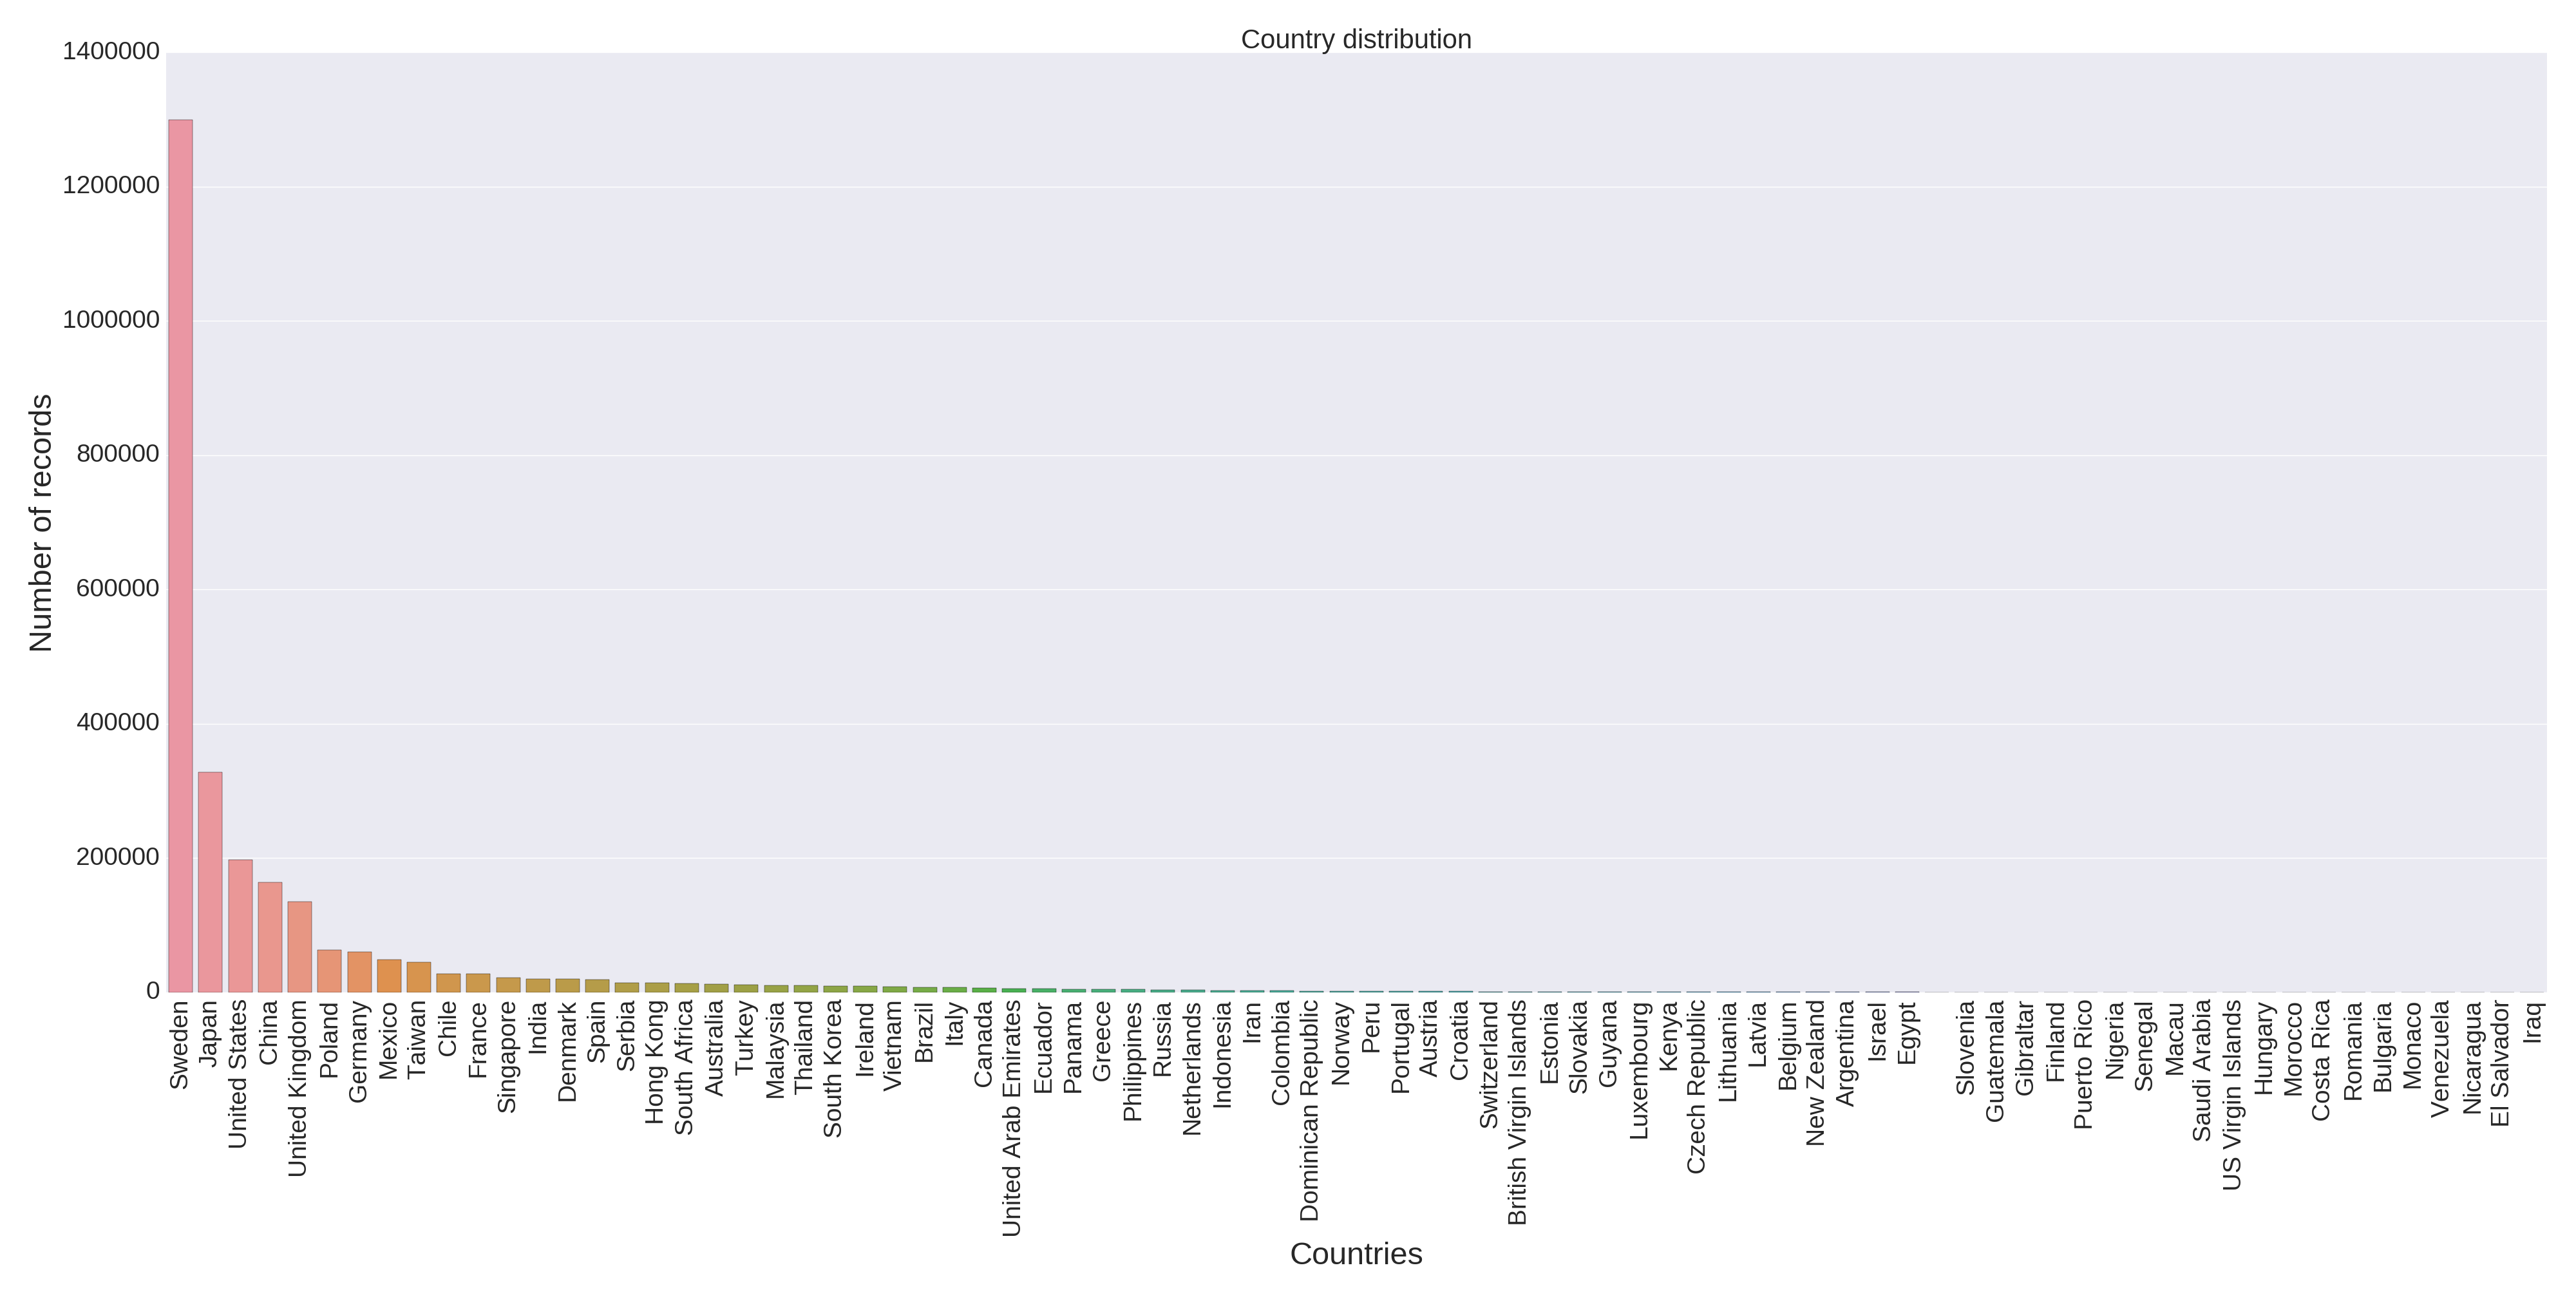
\includegraphics[scale=0.14]{country_distribution}
    \caption{Distribution for number of location updates between countries}
    \label{fig:country_dist}
\end{figure}

At Sverige og Japan er de to størst repræsenterede lande er ikke så mærkeligt, da Sony er et Japansk firma og Sony overtog helt Sony-Ericsson, hvor Ericsson var Svensk. Sony-Ericsson var den gang Sony's mobil mærke. 

På baggrund af Figure \ref{fig:country_dist}, har vi valgt at gå videre med endten Sverige eller Japan. Derfor vil vi nu sammeligne data for de to lande. 
I Japan er der 316 unikke brugere, mens der i Sverige er 542. De to lande kan have brugere tilfælles, da brugerne principielt kan rejse mellem flere lande og derved have lokations opdateringer i flere lande.  
Antallet af totale lokations opdateringer varierer også. Over alle tre måneder har Japan 299,157 opdateringer, hvor Sverige har 1,018,781 opdateringer.

Figure \ref{fig:mean_loc_updates_sep-nov} sammenligner gennemsnittet for lokations opdateringer i Japan og Sverige.
\begin{figure}[H]
    \hspace*{-2.2cm}
    \centering
    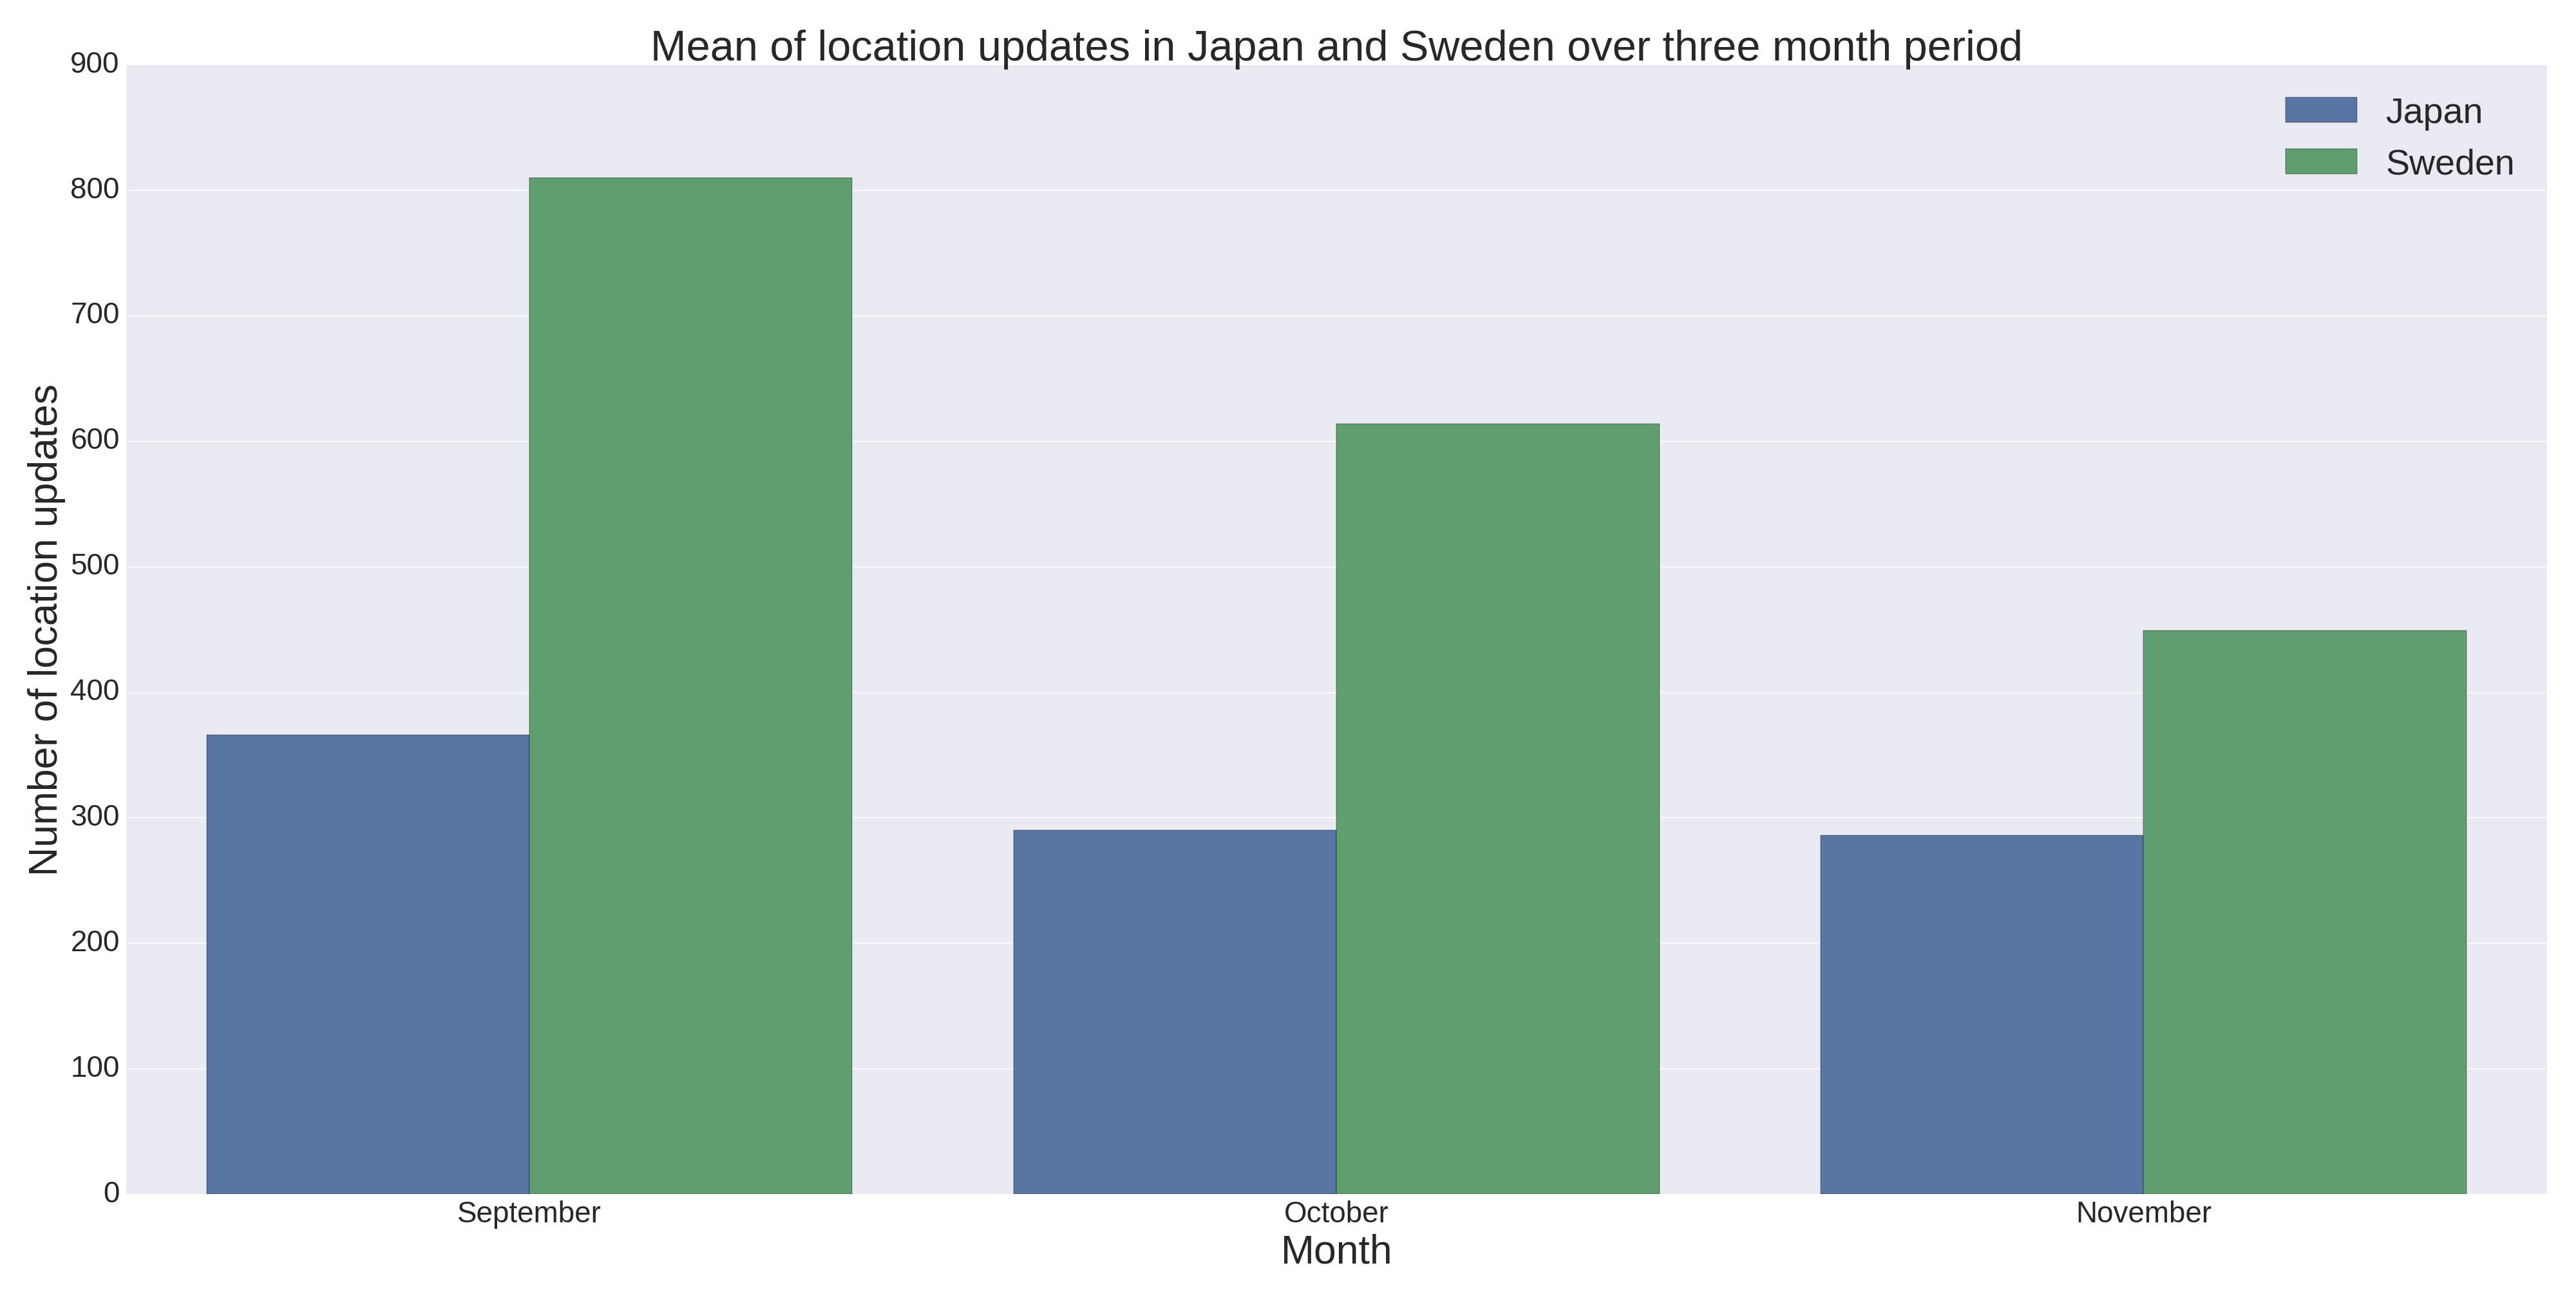
\includegraphics[scale=0.16]{mean_loc_updates_sep-nov}
    \caption{Distribution for mean of location updates for Japan and Sweden}
    \label{fig:mean_loc_updates_sep-nov}
\end{figure}

Vi kan se at Sverige har betydeligt flere opdateringer end Japan i alle tre måneder, hvor landet i September og Oktober endda har dobbelt så mange end Japan. Vi kan også se en nedadgående tendens i begge lande. September har højest antal opdateringer, hvor det herefter går nedad i de to resterende måneder, hvor November for Sverige ligger over 300 opdateringer under September. Selvom tendensen ses tydeligst for Sverige, er den også synlig for Japan. \\
Dette kigger vi nærmere på senere. \textcolor{red}{heatmaps???}



Vi vil gerne se hvordan lokations opdateringerne for de to lande, er fordelt på brugerne. Til dette har vi quantilerne for de to lande, som se i Tabel \ref{tab:stat_loc_updates} 

\begin{table}[htbp]
        \centering
        \small
        \setlength\tabcolsep{2pt}
        \begin{tabular}{|c|c|c|c|c|c|c|c|c|c|c|}
            \hline
                         & Japan      &   Sweden      \\[-1pt]
            \hline
                 Min     &    1       &   1           \\
            \hline
                 Q1      &  22        &   71      \\
            \hline
                 Median  & 251.50     &   902.50      \\
            \hline
                 Mean    &  946.70   &  1,879.70     \\
            \hline
                 Q3      & 1,063.25    &   2,848.25     \\
            \hline
                 Max     &  10,361 &  15,447     \\
            \hline
                 IQR     &  1,041.25   &  2,777.25      \\
            \hline
            
        \end{tabular}
        \caption{Quantiles and mean over location updates for Japan and Sweden} %add this between 'caption' and '{...' for new text in listing of tables: [New caption text only for listing of tables]
        \label{tab:stat_loc_updates}
\end{table}


Hvis vi kigger på landenes quantiler, kan vi se at 25\% quantilen (Q1) er meget lav hos begge lande. Q1 vise med andre ord, at 25\% af brugerne i Japan og Sverige har henholdsvis maksimalt 22 og 71 opdateringer, henover alle tre måneder. Dette er ikke et godt tegn at så mange brugere har så få opdateringer. 75\% quantilen (Q3) er en del højere i Sverige end i Japan, hvilket viser der er 75\% af brugerne der har maksimal 1,063.25 og 2,848.25 lokations opdateringer i henholdsvis Japan og Sverige. Dette ser igen bedre ud i Sverige, hvis brugere har flere opdateringer end Japan. \\ 

Begge lande har en lille procent brugere, som står får utroligt mange opdateringer. I Sverige er der 25\% brugere som har mellem 2,848.25 og 15,447 opdateringer og i Japan har de mellem 1,063.25 og 10,316 opdateringer. Dette er ligesom med Q1 et dårligt tegn. 
Median og mean er meget større i Sverige end Japan. Dette tyder på at der er flere brugere med flere lokations opdateringer i Sverige end i Japan. \\


Den ovenstående tendens, vil vi gerne vise mere tydeligt, hvorfor vi har plottet den Cumulative Distribution Function (CDF) for de to lande. 
\begin{figure}[H]
    \hspace*{-1.0cm}
    \centering
    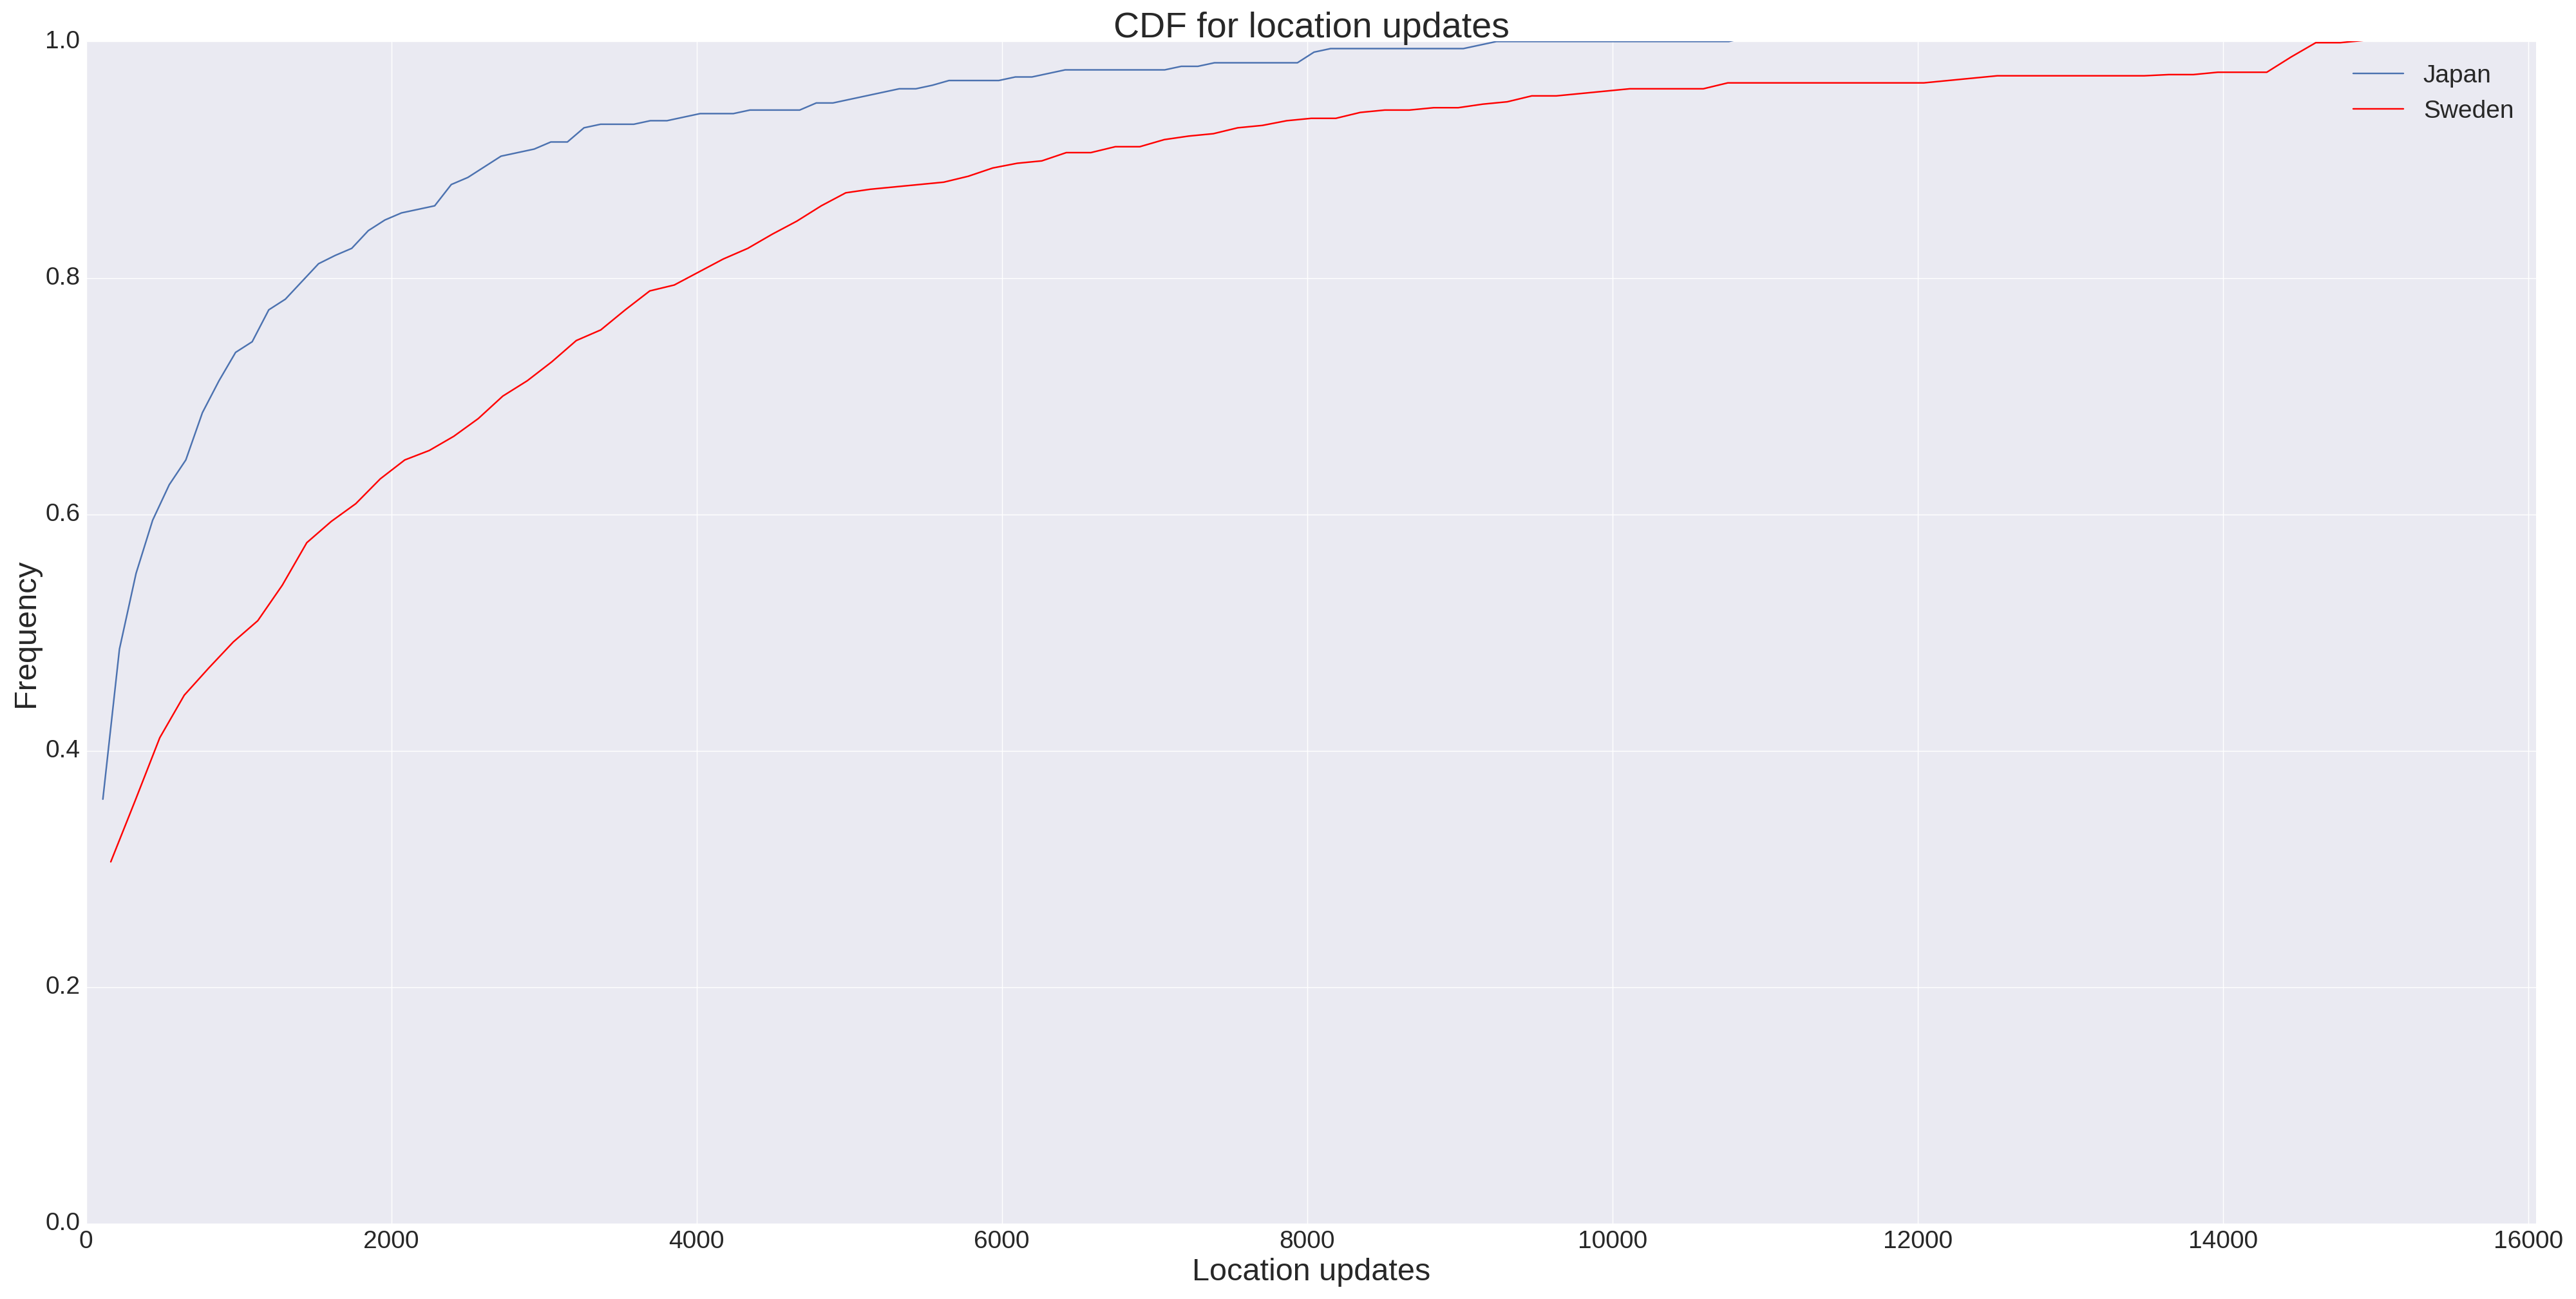
\includegraphics[scale=0.14]{cdf_location_updates_swe_jap}
    \caption{Cumulative Distribution Function (CDF) over location updates for Japan and Sweden henover periodens tre måneder}
    \label{fig:country_cdf}
\end{figure}

Plottet viser, at der både i Japan og Sverige er en stor del af brugerne, som har meget få lokations opdateringer set henover hele perioden. Det kan ses, at Japan får hurtigt flere brugere med få opdateringer, end Sverige. 
Da opdateringerne kommer hver gang brugeren skifter lokation, betyder dette, at mange af brugerene er meget stillestående eller også har de slukket mobilen. Her kan stillestående også menes, at brugeren har glemt sin telefon derhjemme.
Begge disse scenarier tegner ikke godt for vores mål, da det giver sig selv at der skal være nogle data for at finde co-occurences. 
På baggrund af quantiles og CDF, kunne det tyde på at data fra Sverige vil være mere brugbart end Japan. 

Når vi nu ved, at største delen af brugerne i begge lande har få opdateringer, vil vi gerne vide hvodan disse opdateringer er fordelt henover perioden. Det er interssant for os at vide, om opdateringerne er ligeligt fordelt på dagene eller om de klumber sig sammen. Det er interessant, da det kan gøre en forskel med hvad vi bruger til vores modeller. 

Vi har valgt at visualisere dette, ved brug af Heatmaps. 

\newpage


\begin{figure}[H]
    \hspace*{-1.5cm}
    \centering
    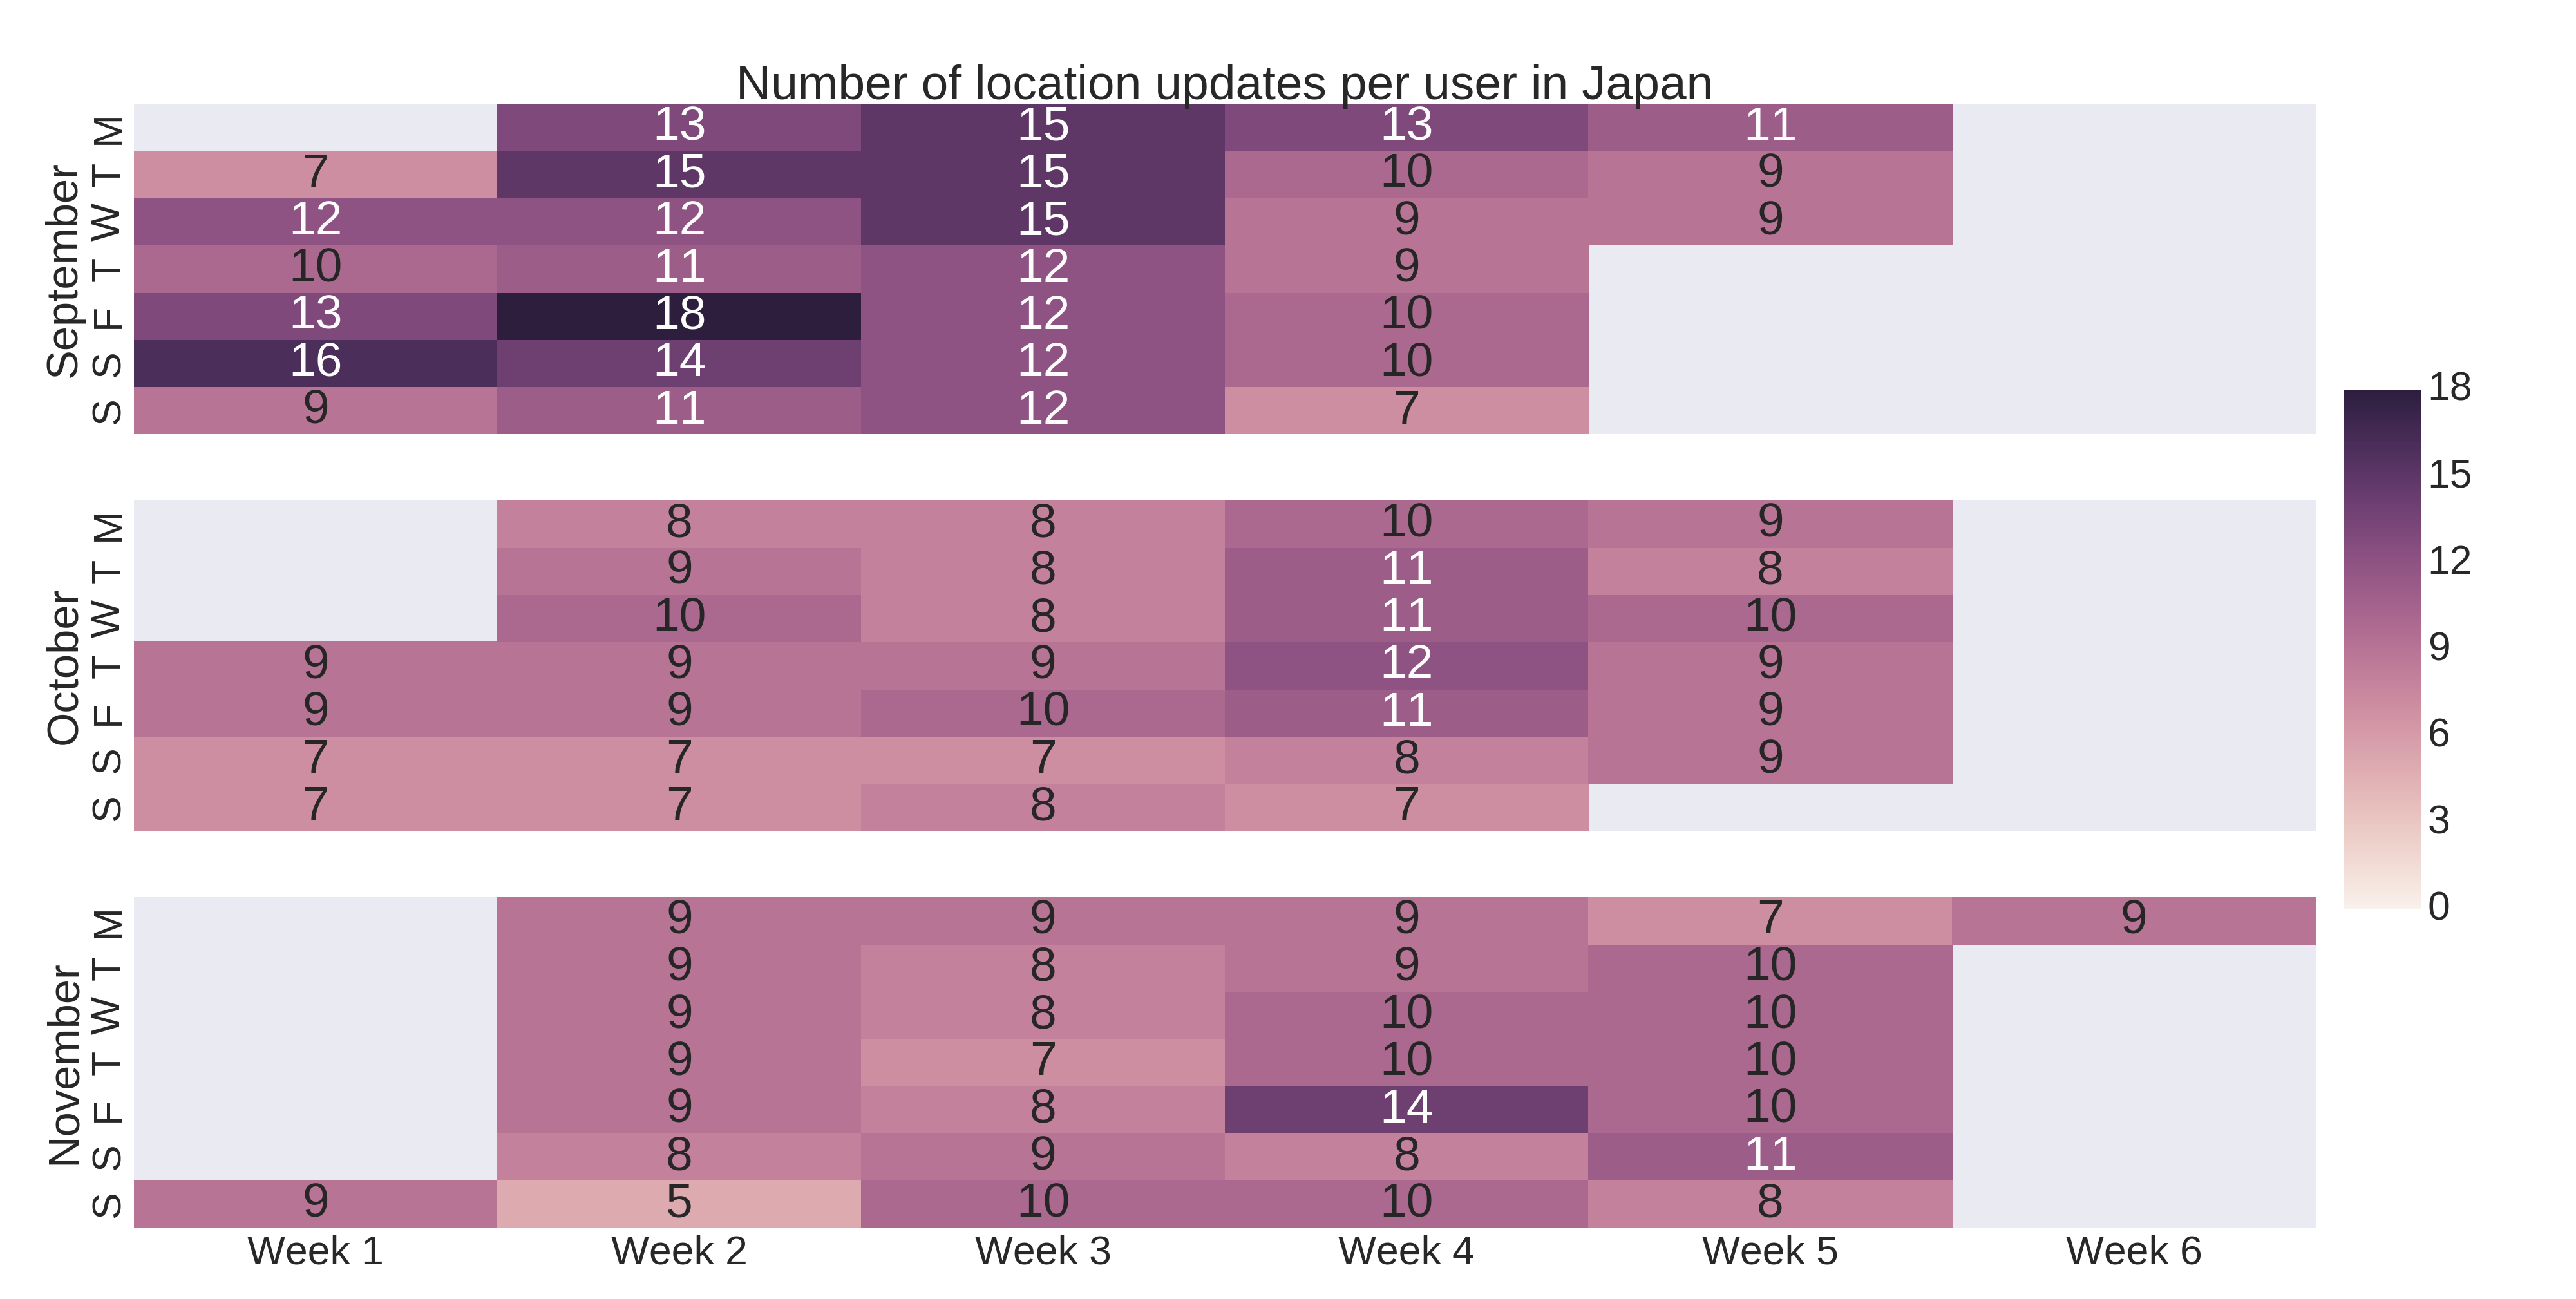
\includegraphics[scale=0.15]{heatmap_location_updates_japan}
    \caption{Heatmap for location updates over the 3 month period in Japan}
    \label{fig:heatmap_jap}
\end{figure}
\begin{figure}[H]
    \hspace*{-1.5cm}
    \centering
    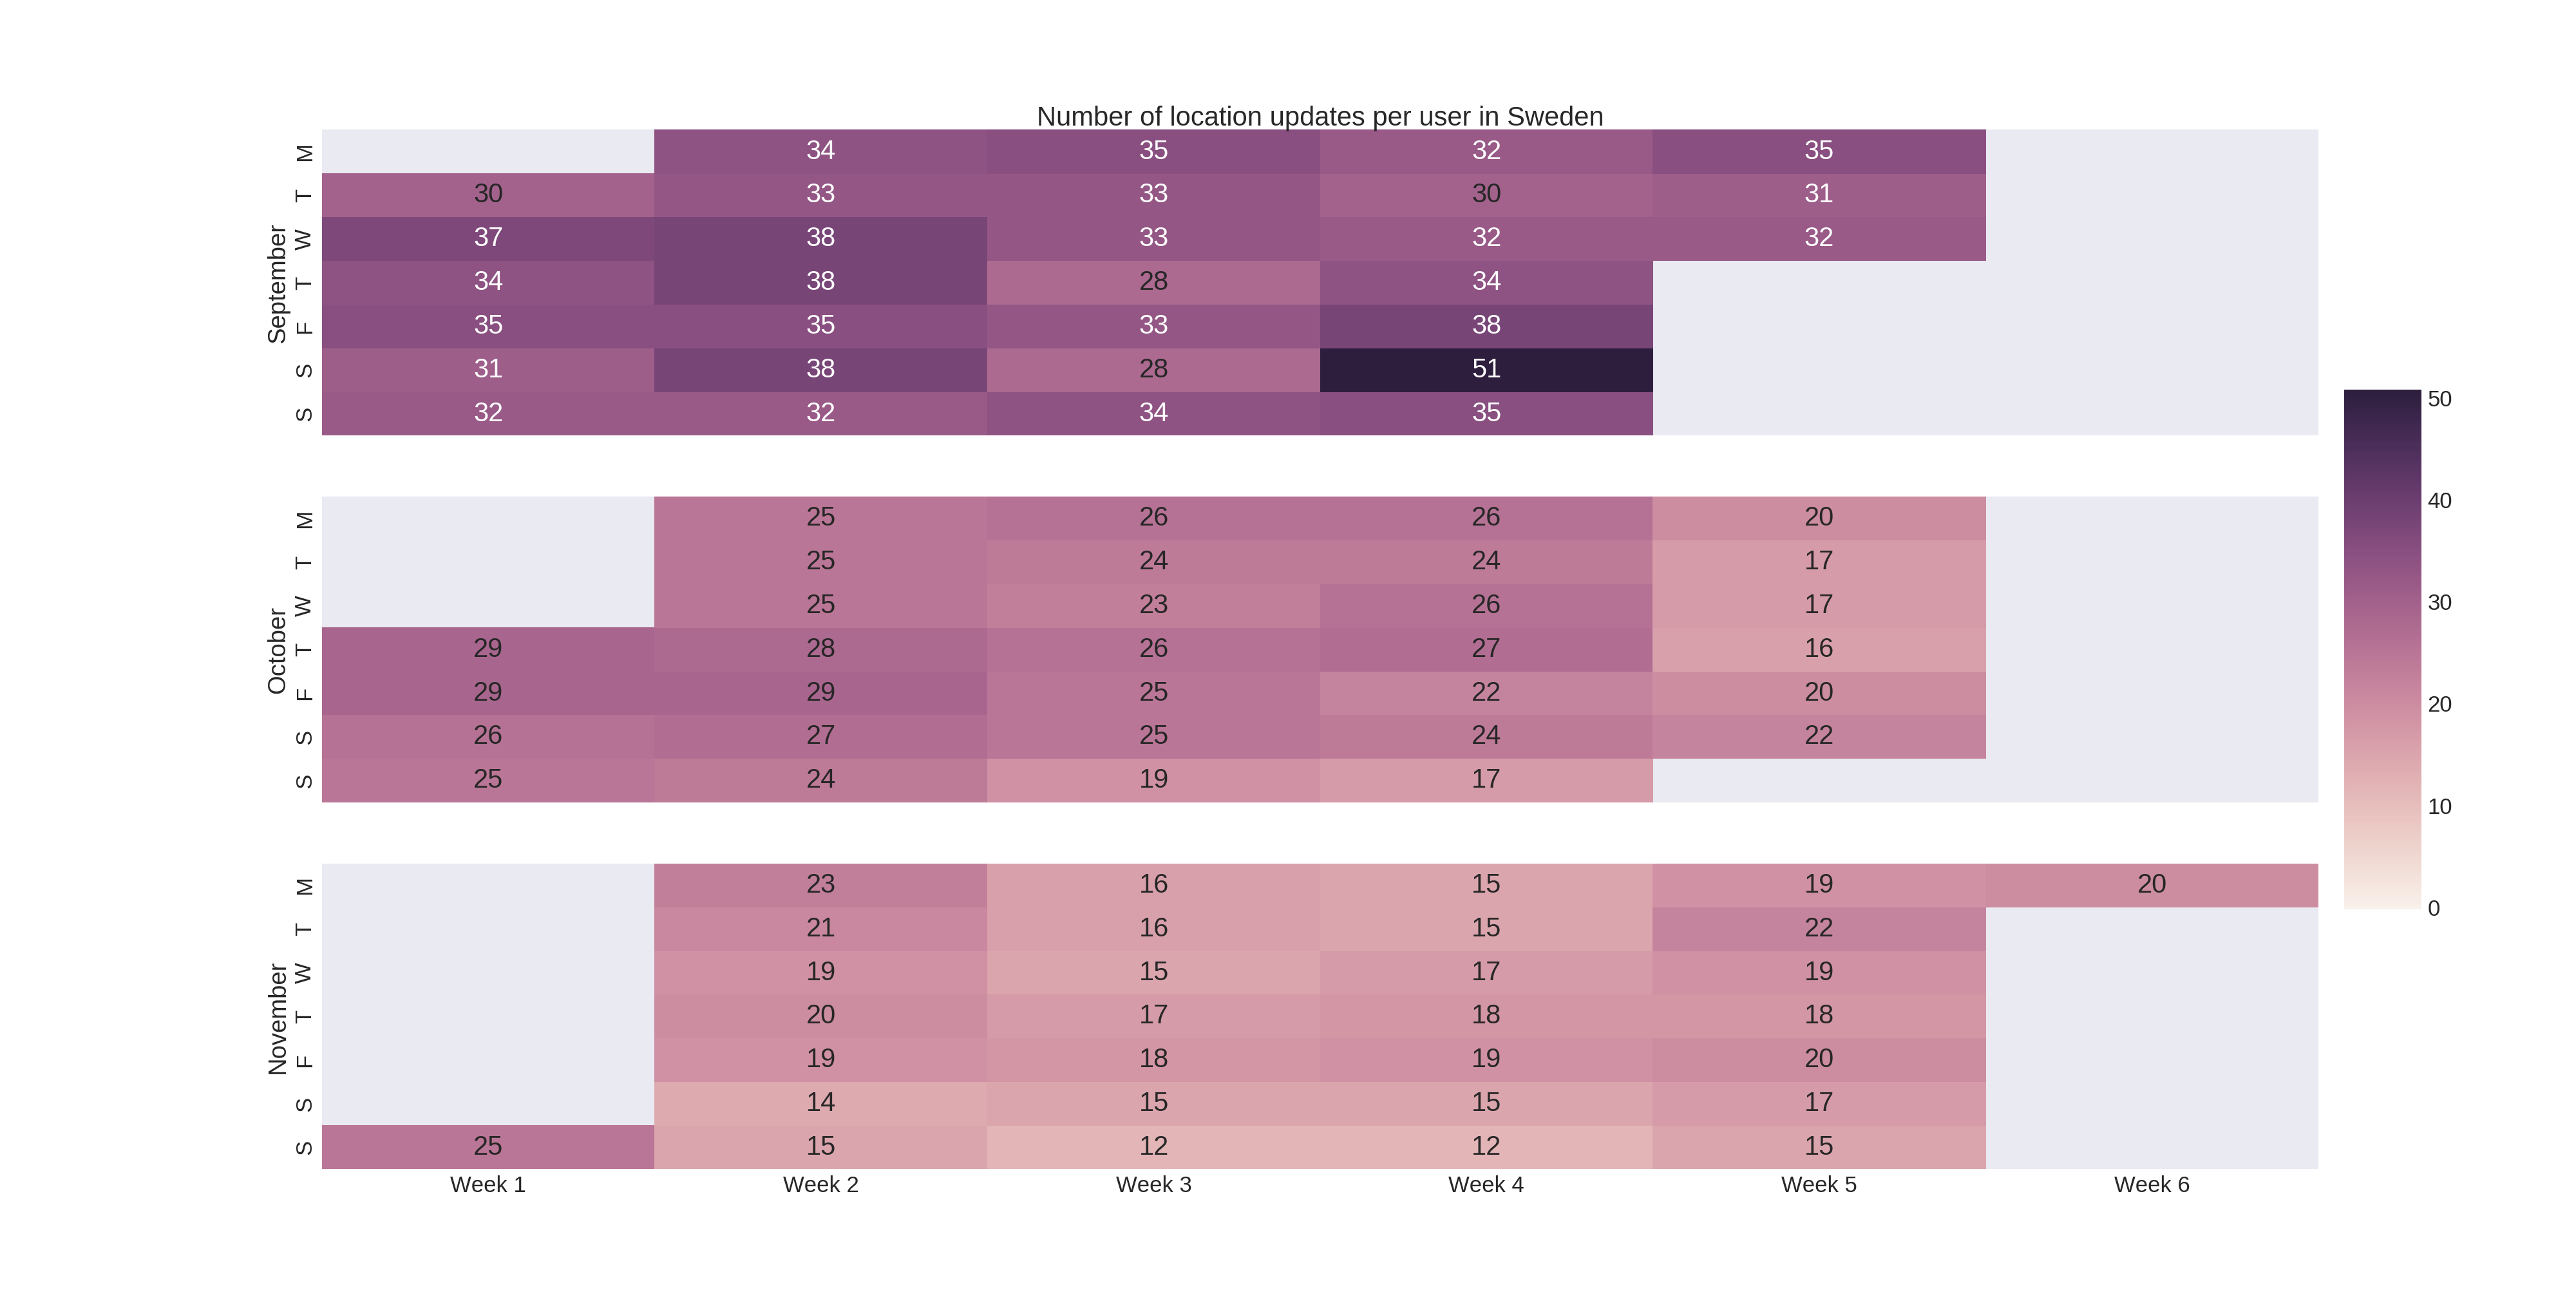
\includegraphics[scale=0.15]{heatmap_location_updates_sweden}
    \caption{Heatmap for location updates over the 3 month period in Sweden}
    \label{fig:heatmap_swe}
\end{figure}


 Figure \ref{fig:heatmap_jap} viser hvordan lokations opdateringerne per bruger (afrundet til heltal) i Japan er fordelt over hver dag i hver af de tre måneder. Figure \ref{fig:heatmap_swe} viser det samme, bare for Sverige. 
 Vi kan f.eks. se, at der i Japan er gennemsnitligt 17 opdateringer per bruger om mandagen i uge 3 i september, hvor der samme dag i Sverige er 35 opdateringer i gennemsnittet. 

 Da alle måneder har samme skala i det enkelte heatmap, er det nemt at sammenligne dagene på tværs af månederne. Vi kan derfor se, at for både Japan og Sverige gælder, at der generelt er mere aktivitet i september, end i da andre måneder. Dette underbygger tendensen fra Figure \ref{fig:mean_loc_updates_sep-nov}, hvor vi kunne se en nedadgående tendens fra september til november. 

 
\newpage


Our work will focus on the location updates from Japan. There is 332 users in Japan for which we have location updates.
When training our classifier we divided the dataset into three parts where each corresponded to a month.

Japan locations for September: 340198
Japan locations for October: 208242
Japan locations for November: 102442

%\subsection{App og homophily del}


Over disse 3 måneder blev der indsamlet 2.665.893 geolokation lokations opdaterings, som er vores primær data. 

When we got the dataset it was stored in three folders, one for each month (9, 10, 11) and within each folder were multiple chunks of data in Apache Avro format\cite{apacheavro}, which we learned is a data serialization framework for Hadoop similar to the JSON format. The chunks were contained in folders bearing the number for each month, however we learned they were sorted by when the server had received the data packet containing the location from the phone and not when the phone had registered the location. The app is storing the collected data on the users phone for a maximum of one month, if the data is not uploaded within a month it is discarded. This approach to data collection means the month folders can contain location updates from the previous month as well.


\subsection{Periode 2}

\subsection{Production data}
\section{Summary}